\subsection{Methodology}

\subsubsection{Waterfall}

{\bf The waterfall process: } is a sequential design process that 'flows' through the phases like a waterfall.
The waterfall process is also known as the 'standard' process because it was the most popular process before
agile processes became popular. 

With the waterfall process do only have a distinct goal for each phase. You can imagine a waterfall on the cliff of a steep moutian. Once the water is flowing over the edge of the cliff, it cannot turn back. It is the same with waterfall development. If you pick the first step of a normal waterfall process you will normally look at the analysis and requirement phase.

{\bf The phases in the waterfall:} there are five main phases in a normal waterfall process. We will here briefly
describe them:
\begin{itemize}
	\item {\bf Requirement specification:} is the phase where you collect all the requirement, functional and non-functional, to make a complete description of the behaviour of the system being developed.
	\item {\bf Design: } is the phase to take the requirements to make a overall design of the system like feks an
	architecture.
	\item {\bf Implementation: } is where the development of the designed system is done. In the implementation phase, 
	it is also normal to do some kind of testing.
	\item {\bf Verification (testing and installation): } when the implementation is done, the solution need to be tested and then installed.
	\item {\bf Maintainance: } is the modification of a software product after delivery to correct faults, to improve performance or other attributes.
\end{itemize}

\begin{figure}[ht!]
\centering
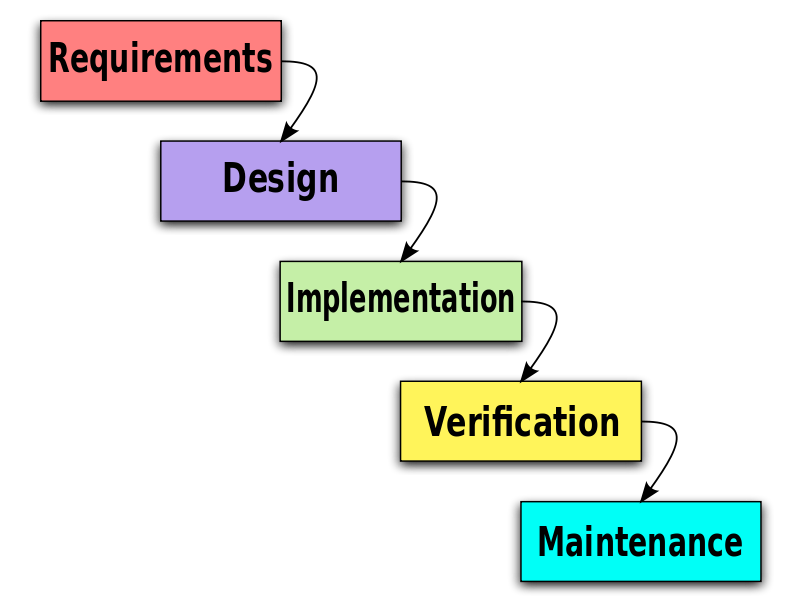
\includegraphics[scale=0.3]{pictures/Waterfall_model.png}
\caption{The waterfall process}
\label{overflow}
\end{figure}

{\bf Pros: }
\begin{itemize}
	\item Simple and easy to understand and use
	\item Phases are processed and completed one at a time.
	\item Works in projects where the requirements are well understood (low risk for changing the requirements)
\end{itemize}

{\bf Cons: }
\begin{itemize}
	\item It is very difficult to change the requirement specification, so it is not suitable for the projects where requirements are at a moderate to high risk of changing.
	\item No delivery of working software until the of the process. This can be critical because the customers may not
	be able to be a part of the process and can entail a unhappy customer.
	\item 

\end{itemize}

{\bf When to use a waterfall process?: }

\subsubsection{Conclusions}


% http://en.wikipedia.org/wiki/Waterfall_model
% http://searchsoftwarequality.techtarget.com/definition/waterfall-model

